\chapter{Trainings- und Validationsdaten}
Zu dem Zeitpunkt, zu dem diese Arbeit verfasst wurde, existierte noch keine Möglichkeit Echtdaten in einem
realistischen Szenario mit einem Mikrocontroller aufzunehmen, der über alle nötigen Sensoren verfügt.
Aus diesem Grund ist es nötig Daten simulativ zu erfassen.
\newline
\newline
Zur Datenerfassung wird der allzweck Robotersimulator CoppeliaSim verwendet \cite{coppeliaSim}.
Mit diesem Simulator werden verschiedene Fabrikszenarien simuliert und dabei verschiedene Sensorwerte erfasst.
Diese werden dann in einem Vorverarbeitungsschritt gefiltert und mit Sensordaten ergänzt, die in CoppeliaSim nicht verfügbar sind.
Zuletzt werden Features extrahiert und die resultierende Datenmenge in Trainings- und Validationsdaten unterteilt.

\section{Simulierte Sensordaten}
Insgesamt wurden vier Routen über 20 Zyklen erfasst, jeweils zwei mal erfasst.
Einmal für Testdaten und einmal für Trainingsdaten, wobei die letzten fünf Zyklen der
Trainingsdaten als Validationsmenge genutzt wird, die außerdem zur Feature-Auswahl genutzt wird.
Dabei wurden alle 50 ms die xyz-, Koordinaten, Beschleunigung und Gyroskopdaten erfasst, sowie Lichtintensität und Metadaten.
Zu den Metadaten gehören Zeitstempel, Beschriftung des Routenabschnitts und Beschriftung des derzeitigen Zyklusses.
Ein Zyklus ist der vollständige Umlauf einer Route.
\newline
\newline
Abbildung \ref{fig:simple_square_labeled} zeigt eine der vier Routen \glqq simple\_square\grqq.
Jede Route ist mit Markierungen für Zyklen und Standorte ausgestattet.
Die Zyklusmarkierung wird genutzt, um die die Datensätze mit deren derzeitigen Zyklus zu beschriften.
Jedes mal, wenn die Sensorenbox diese Markierung überschreitet, wird der Zähler für den Zyklus inkrementiert.
Die Standortmarkierung wird genutzt, um die Datensätze mit dem derzeitigen Routenabschnitt zu beschriften.
Jedes mal, wenn die Sensorenbox diese Markierung überschreitet, wird der derzeitige Wert für Routenabschnitt auf den Wert der Markierung gesetzt.
Dabei werden alle aufgenommenen Datensätze immer mit dem derzeitigen Wert für den Routenabschnitt markiert.
\begin{figure}[h!]
    \centering
    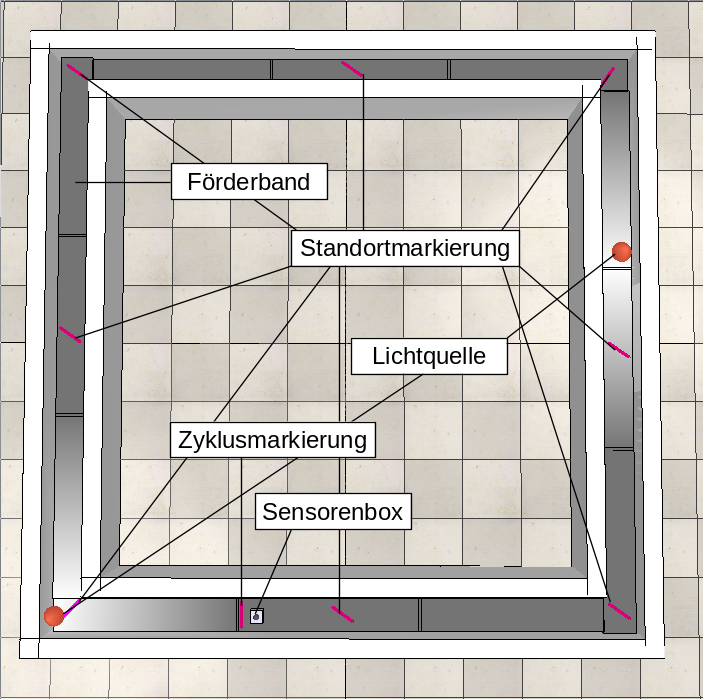
\includegraphics[width=\linewidth]{images/simple_square_labeled.png}
    \caption{Modell der Route \glqq simple\_square\grqq\ in CoppeliaSim mit Beschriftungen.}
    \label{fig:simple_square_labeled}
\end{figure}
\newline
\newline
Neben \glqq simple\_square \grqq\ gibt es noch drei weitere Routen (siehe Abbildungen \ref{fig:long_rectangle}, \ref{fig:rectangle_with_ramp} und \ref{fig:many_corners}).
Die Route \glqq long\_rectangle \grqq\ weist lange Pfade mit wenig Änderungen auf.
Die Route \glqq rectangle\_with\_ramp \grqq\ besitzt zusätzlich zwei Rampen, wodurch Höhenunterschiede simuliert werden.
Die Route \glqq many\_corners \grqq\ ist sehr komplex und hat viele verschiedene Standorte.
Die Förderbänder können verschiedene Geschwindigkeiten haben mit sowohl abrupten Übergangen, als auch fließenden Übergängen zueinander.
\newline
\newline
Je nach Enkodierungsart (siehe Kapitel \ref{sec:model_location_encoding}) müssen die Knoten und Kanten, dieses zyklischen Graphen, als Standorte enkodiert werden.
Als Knoten wird die Menge der Datensätze bezeichnet, die sich in einem Umkreis des ersten Datensatzes befinden, der mit einem Standort beschriftet ist,
d. h. Datensätze mit der gleichen Standortbeschriftung, die sich nicht im Umkreis des initialen Datensatzes befinden, gelten nicht als dieser Standort.
Die Knoten werden mit dem Wert der Standortbeschriftung beschriftet.
Die übrigen Datensätze werden entweder als unbekannten Standort beschriftet oder erhalten einen diskreten Standortwert, der die Beziehung der Kante zwischen zwei Knoten enkodiert.

\section{Künstlichen Sensordaten}
\begin{itemize}
    \item Motivation: Warum ist das nötig?
\end{itemize}

\subsection{Magnetfeld}
\begin{itemize}
    \item Welchen Sensor spiegelt das wieder?
    \item Wie funktioniert das Modell?
    \item Was und Wie wurden Daten ergänzt?
\end{itemize}

\subsection{Temperatur}
\begin{itemize}
    \item Welchen Sensor spiegelt das wieder?
    \item Wie funktioniert das Modell?
    \item Was und Wie wurden Daten ergänzt?
\end{itemize}

\subsection{Lautstärke}
\begin{itemize}
    \item Welchen Sensor spiegelt das wieder?
    \item Wie funktioniert das Modell?
    \item Was und Wie wurden Daten ergänzt?
\end{itemize}

\subsection{WLAN Zugangspunkte}
\begin{itemize}
    \item Welchen Sensor spiegelt das wieder?
    \item Wie funktioniert das Modell?
    \item Was und Wie wurden Daten ergänzt?
\end{itemize}

\section{Simulation von Interrupts}
\begin{itemize}
    \item Motivation => Energieverbrauch, Spiegelung der echten Datenaufnahme, Reduzierung der Trainingsdaten
    \item Wie funktioniert ist?
    \item Wie und Wann bei der Datenverarbeitung wird es gemacht?
    \item So wird bei einer Idle Box auch kein Interrupt erzeugt. (Sneaky Beispiel)
    \item Vorteile bei der Trainingszeit, da weniger Trainingsdaten
    \item Wie gut repräsentiert ist jeder Standort danach? => Graph vorher vs. nachher mit training sampling rate
    \item => Problem: Locations können einfach verpasst werden => Sampling rate?
    \item => Damit alle locations ausreichend in den Trainingsdaten repräsentiert sind, wird eine training sampling rate eingeführt
\end{itemize}

\section{Feature-Extrahierung}
\begin{itemize}
    \item Datenfenster: Realzeit vs. Diskret mittels Wakeups => Es werden immer die letzten 3 Behalten über die die Werte geglättet werden
    \item Relevanz von Zeit => Interrupts, Zeit als Feature, Feature können Zeit Abhängig und Unabhängig sein
    \item Welche Feature werden genutzt? => Abhängig von Feature Importance und wie günstig zu berechnen
    \item Wie werden diese extrahiert?
    \item Welchen Mehrwert verschaffen diese Features?
    \item Welchen Einfluss haben Sie im Hinblick auf Ressourcenbedarf(?), Klassifizierungsgenauigkeit(?), Fehlertoleranz(?)
    \item Rede über Feature Importance, insb. über Permutation Importance => Wie nützlich ist ein Sensor?
    \item Diskrete Distinct Location wird außerhalb verarbeitet => Modell verändern, dass die prev loc in Feature Processing step mit rein geht?
    \item Previous Location, Prev. Distinct Location vs. exponentiell abfallene letzte Orte diskutieren
\end{itemize}

\section{Fehlerhafte/Anomalie Daten}
\label{sec:data_anomalie}
\begin{itemize}
    \item Warum und Wieso?
    \item Welche Fehlerdaten werden eingebaut, was ist deren Begründung?
    \item Was ist eine Anomaly?
    \item Welche Anomalydaten wurden eingebaut?
    \item Welche Features werden zur Anomalierkennung extrahiert? Wie werden sie extrahiert? Wie funktioniert das in der Praxis?
    \item window deviation zu no anamoly data vs normal deviation zum avg
\end{itemize}

\section{Aufteilung der Daten}
\begin{itemize}
    \item Kurz und knapp wie und warum werden die Daten aufgeteilt. => Zyklen
    \item Sollten Trainingsdaten um synthetische Daten ergänzt werden?
    \begin{itemize}
        \item Fault Daten, um das Modell Robuster zu machen
        \item Synthetische Routen => Was ist das? Wie werden sie erzeugt?
    \end{itemize}
    \item Wie viele Trainingsdaten werden benötigt?
    \begin{itemize}
        \item Um KNN zu trainieren?
        \item Um Entscheidungsbaum zu trainieren?
        \item Ggf. Unterschiede klären
        \item (Gehört das schon in eine Evaluation, oder ist das hier okay?)
    \end{itemize}
\end{itemize}